\chapter{Experiments}\label{experiments}
The main experimental can be structured into four parts shown in figure~\ref{fig:process}.
In a preprocessing step, we standaradize the Gutenberg dataset to the new PAN20 format and we clean the Fan-fiction dataset.
Then, we transcribe the datasets using the phonetic transcription methods defined earlier.
The resulting datasets, as well as the original dataset, are then used as the inputs to two widely used Authorship Verification algorithms which are described in more detail in this chapter.
Finally, we analyze the results.

\begin{figure}
  \centering
  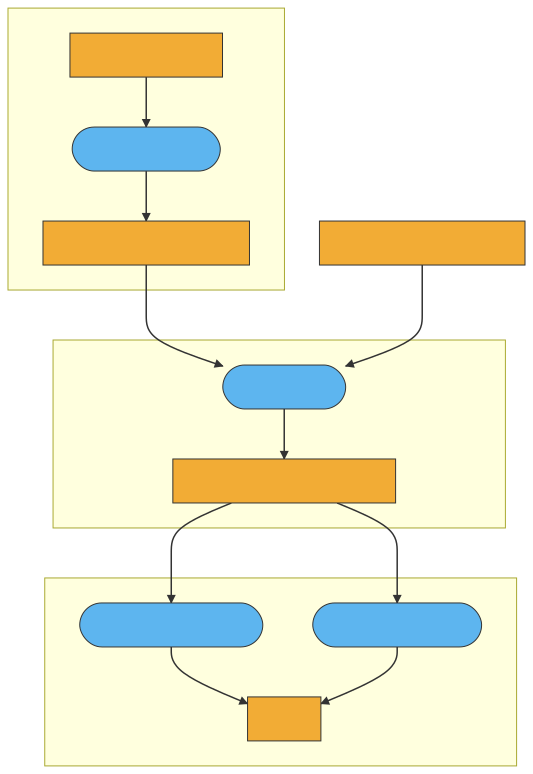
\includegraphics[width=0.6\textwidth]{figures/process}
  \caption{Experimental setup, orange = data, blue = process}
  \label{fig:process}
\end{figure}

% 1.2 Compression Approach
\section{Compression Approach}\label{sec:compression-approach}
The first approach, used as a benchmark in PAN2020 and adapted to Authorship Verification from \cite{teahan2003compression}, uses a text compression method to determine the chance that two texts were written by the same author.
Text compression can be seen as encoding a given text with an encoding that is optimized for this text.
As discussed in \cite{brown1992upperBoundEntropy}, by determining this encoding, text compression can be used to estimate an upper bound to the entropy, i.e., the amount of information of characters in English text.
More specifically, by using the compression model optimized on some text A, the cross-entropy of encoding a text B with this model can be calculated.
During training, this is done for each pair in both directions.
The mean and average of the distance between the resulting cross-entropies are then used to train a logistic regression model.
The smaller the resulting difference, the more similar the texts, and the higher the chance that both are written by the same author.
The compression model used is Prediction by Partial Matching (PPM), a standard algorithm for lossless text compression, first introduced by \cite{cleary1984PPM}.
XXX What is the uncertainty interval used here? We use grid search to find best radius?
The source code used is based on a reimplementation of the Authorship Attribution approach from \cite{teahan2003compression} as part of a reproducibility study in \cite{potthast2016reimplementation}.
The adaption for Authorship Verification stems from PAN20\footnote{\url{https://github.com/pan-webis-de/pan-code/tree/master/clef20/authorship-verification}}.
The source code extending the algorithm to use phonetic features and adding cross-validation functionality is available on GitHub\footnote{\url{https://github.com/torond/teahan03-phonetic}}.
% Add figure, only showing cross-validation side!

% 1.3 Unmasking Approach
\section{Unmasking Approach}\label{sec:unmasking-approach}
XXX What is the uncertainty interval used here?\
Unmasking was first introduced by \citeauthor{koppel2004unmasking} in 2004.
In short, it exploits the degradation of classifier accuracy when removing distinguishing features.
It turns out that removing those features iteratively leads to a faster degradation on text pairs by one author than on those by different authors.
Thus, the algorithm "unmasks" the text pairs and thereby reveals the information needed for classification.\\

% Formal definiton & explanation: unmasking step
This approach comprises two steps: First, a cross-validation method is employed to create the accuracy degradation curves for all training samples.
Secondly, a meta-classifier is trained on the resulting curves to differentiate between same-author and different-author curves.\\
XXX From here on!
For a given pair, the texts are seen to be created by two generative processes $p_1$ and $p_2$.
To compute a curve for a pair, both texts are chunked into parts longer than 500 words without splitting paragraphs.
The 250 words with highest average frequencies in the two texts are used as features.
\textcolor{violet}{TBD: Note bag-of-words approach}
In a 10-fold cross-validation linear SVM models are trained to classify if a chunk belongs to $p_1$ or $p_2$.
The resulting accuracy is noted and the three most influential positive and negative features are removed from the feature set \textcolor{teal}{(Is influential the right word here?)}.
The cross-validation and feature removal are repeated until there are no features left.\\
% meta-learning step
The set of curves is then used to train a meta-classifier linear SVM model.
\textcolor{teal}{Note: Rearrange the following sentences to only cite \cite{bevendorff2019unmaskingShortTexts} once.}
As brought to the point by \cite{bevendorff2019unmaskingShortTexts}, features used are "the curve points, the curves' point-wise first- and second-order derivatives, and the derivatives sorted by steepest point-wise drop" \textcolor{teal}{(Should this be paraphrased rather then quoted?)}.\\
% Adaptation for short texts by Bevendorff et al., how is this different? Which features are actually being used?
Unmasking is one of the most robust Authorship Verification algorithms \textcolor{teal}{(\cite{bevendorff2019unmaskingShortTexts})}.
But as it requires sufficient chunks of no less than 500 words length, it is only applicable for book-length texts.
To counter this, \cite{bevendorff2019unmaskingShortTexts} generalizes the algorithm to accommodate for short texts.
Chunks are generated by oversampling the bag-of-words pool of a given text.
Words from this pool are picked randomly without replacement until a length of 700 words is reached and the pool is reset afterwards.
In total, 30 chunks are generated, which are then used for curve generation as above, with the only exception that the five most positive and negative features are removed instead of only three.
As this approach introduces a significant amount of variance in the resulting curves, the unmasking step is repeated three times and the curves are averaged.
XXX Explain 32 runs!
This time, the meta-classifier uses the curves' "central-difference gradients (first- and second-order), as well as their gradients sorted by magnitude" \textcolor{teal}{(\cite{bevendorff2019unmaskingShortTexts})}.
\cite{bevendorff2019unmaskingShortTexts} also supplies an implementation of the generalized unmasking algorithm which is used as the basis for our research\footnote{\url{https://github.com/webis-de/unmasking}}.\\
\textcolor{violet}{TBD: Explain that we'll use transcriptions with bag-of-words first, then $Dolgo$ with n-grams.}
Note that we only use the Gutenberg dataset for unmasking, as processing the fanfiction dataset would for each of the transcriptions would take multiple weeks.
%We suspect that the differences would not be significant. (Can I phrase that like this??)
We added an out-of-fold cross-validation functionality to the unmasking framework to extract as much information as possible from the much smaller Gutenberg dataset.
The results are then compared to results obtained from verbatim text.
%(Maybe add more code details! What else was added etc.)


% Explain OOF crossval (with diagram?)
% State how many folds are used!
% -> Explain error correction measures
% Maybe: Note run time for (transcription &) algorithms